
\chapter{The Role of Focus in Object Instance Recognition}



% As a general rule, do not put math, special symbols or citations
% in the abstract

We present a study on the effects of focus on object instance recognition (identifying instances of the same object or very similar object, for example a particular product) using Convolutional Neural Networks. The field of object detection is seen as an harder task than that of recognition, as the object must be localised as well as classified. In the field of face recognition, alignment is seen as a crucial step for the purpose of recognition - it is our hypothesis that focus and alignment is similarly important for object instance recognition. 

We perform some experiments to verify the effects of localisation, using datasets with bounding box annotations. We found that CNN classification on images cropped to bounding box regions is much more accurate than classification of whole images. Both magnification and centring of the object in question seem to also have a strong effect, and including context in the classification is only useful if it does not come at the expense of minifying the object to be classified.
 
We conclude in order to produce a quality instance recognition using CNNs for classification, it would be a large advantage to first localise and then focus on the region of interest. Future research will focus on how this localisation can be performed, for example using a model to first estimate a bounding box and rotation using regression, or using Spatial Transformer Networks which enable learning a joint classification and focus method.




\section{Introduction}

Object detection is described typically as a harder problem than object recognition only, for the reason that it requires not only classifying which object is present, also establishing where each object is located. We look at this from another angle, if we can first focus on the location each object is located - can we do a much better job of identifying which object is present? 

Convolutional Neural networks (CNNs) \cite{LeCun1998} have become the tool of choice for image classification problems in recent years. Despite having been invented many years earlier it was the advent of GPUs enabling larger datasets and larger networks which triggered adoption, initially coming to prominence in \cite {Krizhevsky2012}.  We experiment with how focus influences the performance of a CNN model for the purpose of instance recognition. Our interest is in instance recognition, we can see that these ideas are not unique to instance recognition but for object recognition and classification with CNNs in general.

CNNs are said \cite{Krizhevsky2012}, to having properties which make them invariant to translation, and naturally learn redundancy to scale and rotation present in the training data. Is it necesscary then, that CNNs, must be focused and aligned on the exact area of interest? The role of focus and alignment can be seen most clearly in face recognition, where faces are aligned very precisely. Face recognition almost ubiquitously uses alignment as a pre-processing step, before passing images on to a model for recognition purposes even when the model is a deep CNN \cite{Taigman2014}.

It seems intuitive that focusing on the relevant part of an image should produce a better outcome, however we're also aware that the context of an object is said to be important in recognition \cite{Torralba2003}. For example the background of water and sky gives a strong clue that the object is more likely to be a boat than a car. A cluttered background is seen as a problem in object recognition and detection, and it was noticed in an effort to compare image patches, that prioritising pixels in the centre of a patch \cite{Zagoruyko2015} increased performance. In this light -- it is unclear if including context in image classification is always advantageous. 

We look at this in the context of object instance recognition with two datasets where objects have been localised with bounding boxes. We use two instance recognition datasets the Washington RGB-D dataset \cite{Lai2011} of object turntable sequences, and the INSTRE dataset \cite{Wang2015} containing photographs of objects captured by hand. In the case of the INSTRE dataset, most (but not all) objects are captured with backgrounds where context is not very predictive - for example a toy captured with a grassy background. The RGB-D dataset is captured in a controlled environment with a white turntable in the background in all images.

CNNs are frequently used to learn alignment, for example bounding box regression as is common in object detection \cite{Sermanet2013}. In face recognition facial features are commonly detected and used to align the face very closely with other face images, which is also typically performed using a CNN. For the generic task of object instance recognition we don't have the luxury of obvious landmarks for alignment, as they vary largely depending on the type of object, but we can consider more general alignment such as estimating bounding box(es) or using regression to estimate rotation as in \cite {Fischer2015}. 

Spatial transformers \cite{Jaderberg2015a} are another option and enable a joint learning of a classifier and attention method (affine transformation) for CNNs, with evidence they  house numbers in natural images \cite{Netzer2011} and bird species recognition \cite{Wah2011} In future we will evaluate these alignment methods for the purpose of object recognition as well as consider methods of capturing object images with bounds and orientation, if identifying the correct focus is more difficult than recognition there is little point.


\section{Method}

We use the same training method, and optimisation method throughout, except where mentioned the parameters are as described in this section. 

\subsection {Learning}

We use standard Stochastic Gradient Descent (SGD) with momentum set to $ 0.9 $. We set the learning rate to $ 10^{-2} $ and interpolate this rate across each epoch to a minimum of $ 10^{-4} $. We interpolate the learning rate using Stochastic Gradient Descent with Restarts (SGDR) \cite{Loshchilov2016}, however we reduce the learning rate at each mini-batch instead each epoch. We set our epochs to be relatively large accordingly, and restart SGD at the higher learning rate at the beginning of each epoch. 

Each training cycle was performed with epoch sizes of 65536, and 10 epochs were trained in all cases, after which the loss function plateaued. We use a mini--batch size of 64, an image size of $64\times64$ (though this is varied for some experiments). We select images from each class randomly with uniform probability, as well as images from within each class with uniform probability.

\subsection {Network}

We use the same architecture CNN in each case, varying slightly for experiment two where we increase the pixel size of the input image (see below for details). We use a simple AlexNet \cite {Krizhevsky2012} style model, details are given in table~\ref{fig:network}. Other network architectures, such as the popular ResNet \cite{He2015} style were evaluated, and perform very similarly at the tasks presented here, at the expense of taking longer to train.

Each convolution operation is padded, in order that inputs and outputs dimension match (e.g $ 7\times7 $ convolutions have inputs zero padded by 3 pixel, and $3\times3$ convolutions have inputs zero padded by 1 pixel). It can be seen that each layer (ConvLayer) halves the input resolution after convolution, using max-pooling. For a non linearity we use the Parameterised Rectified Linear Unit (PRelU). Batch Normalisation is used directly before all convolution layers and uses a running sum with momentum = 0.9.

Our classification method is the standard SoftMax method with the usual cross entropy loss function. Before the final linear layer we use a single dropout layer $ p = 0.5 $, which we have found prevents over-fitting even though it is said to be unnecessary to use both Batch normalisation and dropout.  We use the Torch7 \cite{Collobert2011} neural network library to implement this network and perform all experiments. 

\begin{table}[h]
  \centering
    \caption{Neural network structure }
\begin{tabular}{ l } 

\toprule

 ConvLayer(n) = PRelU $\rightarrow$ Batch Normalisation \\ 
 $\rightarrow$  Convolution $(3\times3, n \rightarrow n * 1.5)$ $\rightarrow$  Max Pooling $(2\times2)$ \\
\\
 LinearLayer(m, n)  = PRelU $\rightarrow$ Batch Normalisation \\  $\rightarrow$  Linear $(m \rightarrow n)$ \\
\toprule
  Network = Batch Normalisation $\rightarrow$
 Convolution $(7\times7, 3 \rightarrow 32)$ \\
 $\rightarrow$ Max Pooling $(2\times2)$   \\

  $\rightarrow$ ConvLayer (32) $\rightarrow$  ConvLayer (48) $\rightarrow$ ConvLayer (72) $\rightarrow$ ConvLayer (96)   \\
  
  
  $\rightarrow$ Flatten $(2\times2\times144 \rightarrow 576)$ $\rightarrow$ LinearLayer (576, 256) \\
  
  $\rightarrow$ Dropout(0.5) $\rightarrow$ LinearLayer (256, $\vert classes \vert$ )  $\rightarrow$  SoftMax($\vert classes \vert$) \\
  
    
       
\toprule
\end{tabular}

\label{fig:network}
\end{table}




\subsection {Image Preparation and Pre-processing}


\begin{figure*}[t]
    \caption{Examples of data augmentation }
\centering
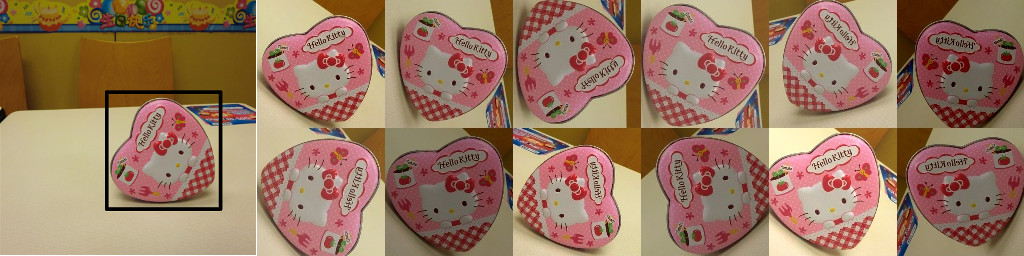
\includegraphics[width=1.0\textwidth]{focus/image_variations.jpg}
\label{fig:variations}
\end{figure*}


In cropping an image to it's object's bounding box, we use a uniform scaling -- in order to ensure the entire object fits within this bounding box we fit a square around the bounding box in the cases where the bounding box is not square (we use square images as inputs to neural networks in this work).

We used data augmentation heavily to regularise the training in the form of random image transformations. Training images are randomly transformed using a set of parameters sampled from a normal distribution and shown in table \ref{fig:jitter}.  We use translations, rotation about the centre, scales (uniform and non uniform), brightness and contrast adjustments. Testing images are resized and cropped in the same way (described below), but with no random transformations. An example of training data is given in figure~\ref{fig:variations}.

\begin{table}[h]
  \centering
    \caption{Ranges of parameters used for image distortion }
    
  \begin{tabular}{ l  l }
    Parameter & Mean $ \pm $ Standard deviation \\
    \toprule
    scale (uniform) & $ 1 \pm 0.2 $  \\ 
    non uniform scale  & $ 1 \pm 0.2 $  \\ 
    rotation (degrees) & $ \pm 90 $ \\ 
    translation(x, y) (\% image size) & $ \pm 5 $ \\ 
    brightness (additive) & $ \pm 20 $ \\ 
    contrast (multiplicative) & $ 1 \pm 0.2 $ \\ 
    \bottomrule
  \end{tabular}
\label{fig:jitter}
\end{table}


An affine transformation matrix $ (2 \times 3) $ is computed, firstly scaling the image to fit the bounding box region to match the network's input size, applying a set of random transformations as above, then cropping a rectangular region around the origin of the transformed image. We use OpenCV's warpAffine function to perform this as a single step, avoiding artefacts from multiple image transformations (and also to avoid having to compute intermediate images with associated clipping issues).

\subsection{Datasets}

The RGB-D \cite{Lai2011} dataset which contains turntable images with a fixed camera at 30 degrees, 45 degrees and 60 degrees of elevation. For evaluating instance recognition the 30 and 60 degree images are used for training, and the 45 degree images used for testing. Bounding boxes are provided for each image (generated using depth information). The RGB-D dataset contains approximately 500 images (varying a little) for each instance, with 300 different object instances. We make no use of the depth images provided in the dataset.

The INSTRE \cite{Wang2015} aims to be a more diverse, better balanced dataset with cluttered backgrounds than existing object instance recognition datasets. It improves on the RGB-D dataset in that the range of views are much more varied, the types of object have more variety, the backgrounds have variety (hand taken photos) rather than the turntable background. Bounding boxes are again provided. No standard test set is provided for the INSTRE dataset, so we take every 4th image of each object for testing, and use the remaining images for training. The INSTRE dataset contains 200 classes of object, each with 100 images which have either been hand captured or picked. 

The INSTRE dataset contains unique challenges. A number of the objects are a little abstract, and include things like logos (e.g. one of the categories is KFC, which includes pictures of the building prominently showing the logo, as well as napkins containing the logo and pencil drawings). An example hard case is shown in figure~\ref{fig:adidas}. Many categories feature objects rotated in numerous ways, with both landscape and portrait images, as well as many photos taken on angles with no alignment at all.

\section {Experiments}


\subsection {Experiment 1}

Our first experiment compares the effect of focusing on the bounding box on classification accuracy. If we had an oracle which could give us a bounding box estimate (or another model which could accurately give a bounding box estimate) - how much better is the network performance on cropped versus baseline (uncropped) images? We apply this cropping equally on test and training images.

For the RGB-D dataset, which for many of the objects only occupy a tiny space of the full image, we crop the inner centre 40 percent of the image for the uncropped baseline. Otherwise, after scaling the original image to $ 64 \times 64 $ the smaller objects occupy only a few pixels, with the turntable and background being vastly bigger in scale. In order to see if the magnification from cropping to the bounding box was having an effect, we also ran the baseline at a higher resolution - but noticed little change in performance.


\begin{table}[h]
  \centering
    \caption{Cropped vs. uncropped images }
    
  \begin{tabular}{ l l l }
    
    Dataset & Image preparation & test set accuracy \\
    \toprule
    
    INSTRE & baseline &  65.3 \\
    INSTRE & bounds cropped & 89.0 \\
    
    RGB-D & centre cropped & 58.1 \\
    RGB-D & bounds cropped & 81.6 \\
    
    \bottomrule
  \end{tabular}
\label{fig:crop}
\end{table}

The RGB-D results suggest over-fitting, with the training accuracy reaching almost 100 percent, yet generalising badly to the test set. The RGB-D images present a problem in that the test set (those images captured at 60 degrees elevation), are from a slightly different distribution from the training (they're captured at a constant level of elevation). Each image is also reasonably redundant due to being part of a video sequence. A potential solution to this is using a higher level of randomised non uniform scaling when training. The INSTRE images on the other hand have no systematic difference between training and test images and also cover a much greater intra--object variety and do not show the same kind of over-fitting.

It is clear that focussing on the bounding box has a large impact on the performance of the classification, with both RGB-D and INSTRE classification improved when trained and tested on images cropped to the bounding box. Given this is the case, we seek to discover exactly why. Which property which enables effective classification using this kind of CNN model? Is it the magnification of the object after cropping an image to the bounding box or removing the distracting background? (It is clear the object is much larger in pixels after the resulting image is scaled to match the CNN input size). Or is it the centring of the object, suggesting the translation invariance of the CNN is not as general as is widely assumed?


\subsection {Experiment 2}

\begin{figure*}[t]
    \caption{Examples of cropping for context}
\centering
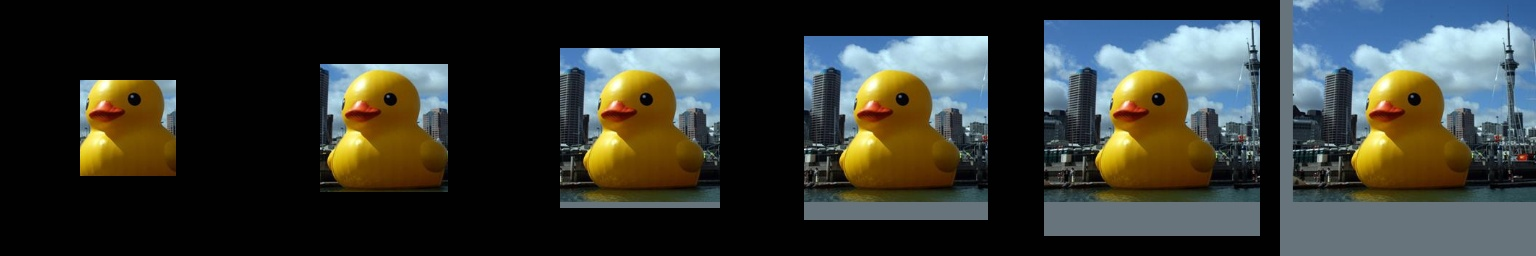
\includegraphics[width=1.0\textwidth]{focus/enlarge.jpg}
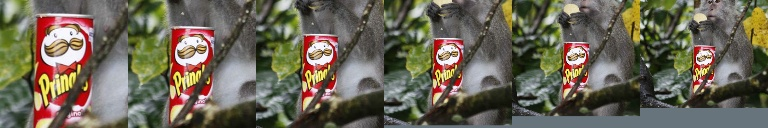
\includegraphics[width=1.0\textwidth]{focus/shrink.jpg}
\label{fig:context}
\end{figure*}




\begin{figure}[h]
    \caption{Context in image classification vs. test set accuracy}
\centering
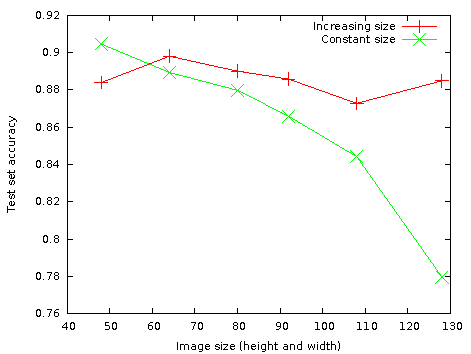
\includegraphics{focus/graph.pdf}
\label{fig:exp2}
\end{figure}

For our second experiment we explore how including context changes the performance. We do this in two ways, firstly by fixing the pixel size of our object and including more context by using a larger input image to the model, secondly by fixing the size of the input to the network and including the same context, where the object is scaled down to accommodate.

In the first case we scale the object bounding box to $ 64 \times 64 $ and set this as the base scale, each larger size includes proportionally more context where the object remains a constant size in pixels. In the second case we use a fixed image size of $ 64 \times 64 $, using the same image context for each size as the first case, causing the object to be relatively scaled smaller.

The architecture of the network is mostly unmodified (each image output within the hidden convolutional layers in the network is of a larger dimension). The number of parameters is constant for the convolutional layers, but the first fully connected layer contains a larger number of inputs to cope with the extra outputs from the convolutional part. The differences can be seen in table~\ref{fig:sizes}.


\begin{table}[h]
  \centering
    \caption{Example output sizes for input dimensions }
\begin{tabular}{ l l l } 
 
 \toprule
 Input image size & Convolution outputs & Flattened size \\
 \toprule
 
 $ 48 \times 48 \times 3 \rightarrow $ & $ 1\times1\times144 \rightarrow $ & 144 \\
 $ 64 \times 64 \times 3 \rightarrow $ & $ 2\times2\times144 \rightarrow $ & 576 \\
 $ 108 \times 108 \times 3 \rightarrow $ & $ 3\times3\times144 \rightarrow $ & 1296 \\
 $ 128 \times 128 \times 3 \rightarrow $ & $ 4\times4\times144 \rightarrow $ & 2304 \\
 
\end{tabular}
\label{fig:sizes}
\end{table}

We can see from the data shown in figure~\ref{fig:exp2} that performance is relatively constant where the scale of the object is fixed. Adding context neither gives a performance boost nor hinders recognition (only takes longer to train). Where context is added at the expense of the object scale we can see that at the higher levels the test accuracy drops.


\subsection {Experiment 3}

Given the results from experiment~2, it seems that reducing the scale of the object (in pixel size) causes a degradation of the performance. Experiment~1 shows that the unmodified INSTRE images are still much more difficult to classify for a CNN. Experiment 2 normalises scales between objects (for example.e. the statue of liberty becomes the same size in terms of image pixels as a can of cola). For experiment 3 we use the bounding box to centre the object, but leave the scale unmodified.


\begin{table}[h]
  \centering
    \caption{Effect of input size and centring}
    
  \begin{tabular}{ l l l l }
    
    Dataset & Input size & Test set accuracy \\
    \toprule
    
    INSTRE &  $ 64 \times 64 $ & 65.3 \\
    INSTRE &  $ 128 \times 128 $  & 71.7 \\
    INSTRE &  $ 192 \times 192 $  & 76.0 \\
    
    \toprule
    INSTRE (centred) &  $ 64 \times 64 $ & 71.6 \\
    INSTRE (centred) &  $ 128 \times 128 $  & 80.6 \\
    INSTRE (centred) &  $ 192 \times 192 $  & 84.2 \\
    
    
    
    \bottomrule
  \end{tabular}
\label{fig:input_size}
\end{table}



We can see from this experiment that both increasing magnification, as well as centring the object both give significant accuracy boosts, not to the same level as cropping to the bounding box, but close. Perhaps even larger magnification would be fruitful. 

The fact that centring the object makes such a difference is surprising, given the translation invariance of the CNN architecture, however it is not clear exactly how much a CNN is translation invariant (even though we can see that the filters used in a convolution step are clearly translation invariant - it is not obvious that the network as a whole possesses such properties). A recent study attempting to quantify this translation invariance \cite{EricKauderer-Abrams2016} suggests the architecture, and data augmentation are both important here. 


\subsection {Failure cases - discussion}


\begin{figure*}[t]
    \caption{Example of one hard case in the INSTRE dataset}
\centering

\includegraphics[width=1.0\textwidth]{adidas.jpeg}
\label{fig:adidas}
\end{figure*}



\begin{table}[h]
  \centering
    \caption{Worst categories in testing }
  \begin{tabular}{ l l }
  wangzai & 46.6 \\
  einstein bros & 46.6\\
  Manneken Pis & 45.4\\
  mastermind JAPAN & 45.1\\
  clapperboard & 43.2\\
  Che Guevara & 38.2\\
  coca cola & 33.3\\
  Paul Frank Julius & 32.4\\
  Kung Fu Panda & 24.0\\
  Adidas Originals & 17.2\\
    \bottomrule
  \end{tabular}
\label{fig:failure}
\end{table}

It can be seen in figure~\ref{fig:failure}, that many of the worst performing object classes were those which are somewhat abstract, for example logos which were styalistically the same logo but appeared visually quite different with different colours, materials and occurring in very different contexts. An example is shown in figure~\ref{fig:adidas} for the ``Adidas Originals'' object.



\section{Conclusion}

We found that CNN classification on the cropped bounding box regions is much more accurate than classification of whole images. Both magnification and centring of the object in question seem to have a strong effect (which is somewhat surprising, given the translational invariance properties of CNN models). On the experiments we performed, including context in the input images was only useful if it does not come at the expense of minifying the object (reducing it's pixel size) to be classified.

We conclude in order to perform quality instance recognition using CNNs for classification, it would be a strong advantage to first localise the region of interest, and then focus on the region of interest.  In future we will both further investigate why we see the results above, and at the same time peruse how focus methods can be used to improve instance recognition. Understanding the failure modes in unfocussed image classification is also of interest, understanding in more depth our observations. For the INSTRE data set, the more abstract categories were among those which failed to generalise well, and RGB-D dataset simply over-fit badly.

We will explore bounding box regression as is used in many object detection methods, as well as rotation regression for the purposes of aligning input images to a canonical orientation. One difficulty with using regression is the requirement that your training data requires annotation, making it's use in practice more expensive to obtain. Alternatives include using using external data, and using methods of semi-automated segmentation (for example using a green screen). Alternatively, the use of Spatial Transformer networks is interesting -- which require no such annotation, which jointly learn the focus method with the classifier.




